\documentclass[12pt,a4paper]{article}

\usepackage[utf8]{inputenc}
\usepackage[T1]{fontenc}
\usepackage{lmodern}
\usepackage[margin=1in]{geometry}
\usepackage{graphicx}
\usepackage{booktabs}
\usepackage{longtable}
\usepackage{array}
\usepackage{enumitem}
\usepackage{hyperref}
\usepackage{float}

\setlength{\parskip}{0.5em}
\setlength{\parindent}{0pt}
\hypersetup{colorlinks=true,linkcolor=black,urlcolor=blue}

\begin{document}

\begin{titlepage}
    \centering
    {\large National University of Science and Technology POLITEHNICA,
    Bucharest\par}

    \vfill

    {\LARGE Fetițele Powerpuff - Project Evaluation\par}
    \vspace{0.8cm}
    {\Huge\bfseries Secure Medical OCR Platform with AI-Governed CI/CD\par}
    \vspace{1.2cm}

   \begin{tabular}{>{\centering\arraybackslash}p{0.42\textwidth}
   >{\centering\arraybackslash}p{0.46\textwidth}}
        Andrei-Cristian Airinei & Team Lead and Software Engineer \\
        Ecaterina-Ioana Mincă & Security Software Engineer \\
        Maria Sfîrăială & Android Software Developer \\
        Maria Teodor & Security Software Engineer \\
        Valentin-Ionuț Bobaru & Security Software Engineer \\
    \end{tabular}

    \vfill
    {\LARGE Secure Systems\par}
\end{titlepage}

\section{Project Summary}
\subsection{Overview}
This project is a web platform designed with security in mind, with the
 purpose of using optical character recognition (OCR) for automated 
 processing of medical documents such as occupational health and safety 
 certificates. Since the system processes protected health information (PHI), 
 the traditional, perimeter-only defense model is replaced by a comprehensive 
 Threat Analysis and Risk Assessment (TARA) framework. The entire software 
 development lifecycle (SDLC) is driven by an AI-Assisted, Security-Optimized 
 CI/CD Architecture, enforcing an absolute human-in-the-loop (HITL) 
 deterministic control gateway before any code modifications enter production. 
 The system captures images from mobile clients, sends them through MQTT over 
 mTLS, processes OCR in an isolated service, stores encrypted medical 
 fields in PostgreSQL, and exposes role-protected reporting APIs and 
 dashboards.

\subsection{OSSF Criticality Score}
A run of the OSSF Criticality Score tool resulted in a score of 0.22/1, where 0
means least critical and 1 the most critical. This suggests that our Github
project has a good score and has a low risk.
\newpage


\section{Functionality}

\subsection{Data Ingestion and Secure APIs}
    \subsubsection{Secure MQTT Broker for Medical Files}
    The ingestion channel is based on MQTT with transport security and
    constrained broker behavior. Mobile clients publish captured medical images
    to dedicated topics, while server-side consumers process messages
    asynchronously. Broker configuration applies practical anti-abuse controls
    (connection limits, queue limits, inflight limits, and payload size
    restrictions) to reduce denial-of-service impact while preserving near
    real-time delivery.

    Implemented backend topic map:
    \begin{itemize}[leftmargin=*]
        \item \texttt{ssproject/images/\#} for incoming device images.
        \item \texttt{register/\#} for device registration payloads.
        \item \texttt{auth/login/\#} for MQTT login requests.
        \item \texttt{device/id/\#} for disconnect/inactive updates.
    \end{itemize}

    Example end-to-end usage:
    \begin{enumerate}[leftmargin=*]
        \item Device performs HTTP login and obtains a JWT.
        \item Device sends MQTT registration payload on
        \texttt{register/\{device\_id\}} with token.
        \item Backend validates token, links device to user\_email, and marks
        the device active.
        \item Device publishes image on
        \texttt{ssproject/images/\{device\_id\}}.
        \item Backend verifies device ownership before accepting image.
    \end{enumerate}


    \subsubsection{Secure Web Endpoints}
    The web API exposes authentication, photo management, device information,
    and analytics/reporting endpoints. Access control is JWT-based, with
    role-aware behavior for admin-only operations (for example, anonymized
    export and aggregate reporting views). This enforces a clear separation
    between regular-user data visibility and privileged analytics capabilities.


\subsection{Intelligent OCR Processing}
    \subsubsection{OCR Service Architecture}
    OCR runs in an isolated service separated from the main API and integrated
    through service-to-service calls. This separation improves fault containment
    and allows dedicated hardening of the OCR runtime (restricted container
    profile, non-root execution, and minimal runtime surface). The pipeline
    receives document images, extracts structured text fields, and returns
    normalized outputs for persistence and review.
    Example OCR processing flow:
    \begin{enumerate}[leftmargin=*]
        \item Incoming image bytes are sent to OCR gRPC
        \texttt{ExtractText}.
        \item Backend receives extracted text and marks
        \texttt{ocr\_success} based on non-empty output.
        \item If OCR fails, text is set to \texttt{"OCR failed"} and
        success is set to false.
    \end{enumerate}

    \subsubsection{Standardized JSON Output Schema}
    OCR outputs are normalized into a structured JSON schema used consistently
    across storage, API responses, and UI rendering. Each extracted field
    carries both semantic value and review metadata (confidence, manual-edit
    flag, and validation status), enabling downstream analytics and
    quality-control workflows without schema conversion.
    Implemented extracted medical fields include:
    \begin{itemize}[leftmargin=*]
        \item Identity fields: \texttt{nume}, \texttt{prenume}, \texttt{cnp}.
        \item Employment fields: \texttt{societate\_unitate},
        \texttt{profesie\_functie}, \texttt{loc\_de\_munca}.
        \item Control fields: \texttt{tip\_control} and
        \texttt{control\_*} booleans.
        \item Medical decision fields: \texttt{aviz\_medical} and
        \texttt{aviz\_*} booleans.
        \item Date fields: \texttt{data}, \texttt{data\_urm\_examinari}.
    \end{itemize}

    \subsubsection{Confidence Thresholding and Manual Review}
    Low-confidence extraction is handled through a human-in-the-loop flow.
    Fields below the configured threshold are visually emphasized in the client
    interface, where operators can edit values and explicitly validate them.
    This combines automation speed with controlled correction paths for
    sensitive medical data.

\subsection{Dynamic Reporting and Relational Storage}
    \subsubsection{Database Structure}
    Processed records are stored in PostgreSQL with a hybrid model: relational
    metadata columns (identifier, timestamp, device/user context, OCR status,
    latency) plus structured medical payloads. Sensitive OCR text and medical
    JSON are encrypted before persistence to support confidentiality
    requirements while preserving approved reporting capabilities.
    Storage behavior in implementation:
    \begin{itemize}[leftmargin=*]
        \item OCR text and medical JSON are encrypted before DB save
        (AES-GCM).
        \item Data is decrypted on read before response to API clients.
        \item Image files are stored on disk under
        \texttt{uploads/photos/\{id\}.jpg}.
    \end{itemize}

    \subsubsection{Reporting}
    The reporting layer is implemented as dedicated API endpoints and dashboard
    widgets.
    \begin{itemize}[leftmargin=*]
        \item Alerts for expired medical check-ups. 
        \item Medical insights and status distribution indicators.
        \item Performance metrics for OCR processing latency and success rate.
        \item Anonymized dataset export for controlled sharing.
        \item Expiry alerts for documents approaching renewal deadlines.
        \item Fit by profession, overdue checks, and monthly trend analytics.
    \end{itemize}


\begin{figure}[H]
    \centering
    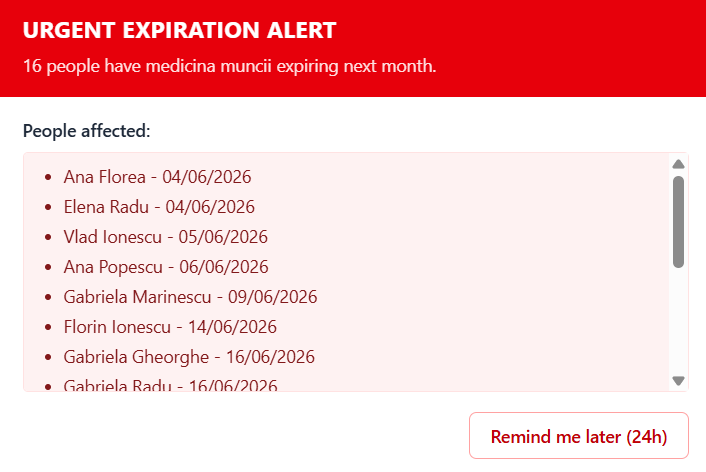
\includegraphics[width=0.9\textwidth]{assets/alert.png}
    \caption{Alert for expiring occupational medicine check-ups}
    \label{fig:expiry-alert}
\end{figure}

\begin{figure}[H]
    \centering
    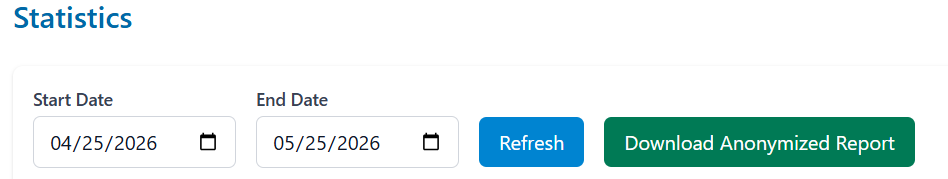
\includegraphics[width=0.9\textwidth]{assets/anon_button.png}
    \caption{Anonymized dataset generation button}
    \label{fig:anon-button}
\end{figure}

\begin{figure}[H]
    \centering
    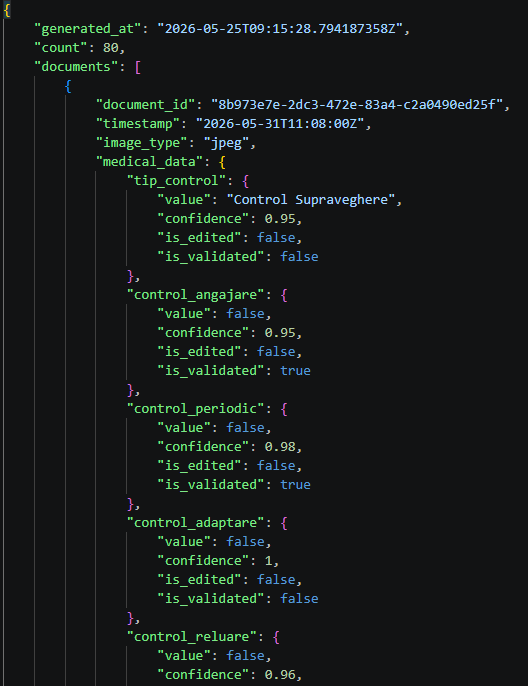
\includegraphics[width=0.9\textwidth]{assets/anon_data.png}
    \caption{Anonymized dataset example}
    \label{fig:anon-data}
\end{figure}

\subsection{Mobile Functionalities}
    \subsubsection{Image Capture Using Device Camera}
    The Android client uses the device camera to capture medical documents
    directly from the field. Capture settings are exposed in the UI to support
    quality/throughput trade-offs, and images are prepared for immediate secure
    upload or deferred transmission in unstable network conditions.
    Example usage:
    \begin{enumerate}[leftmargin=*]
        \item User logs in from Setup screen (email/password) and configures
        broker IP/port.
        \item User enables Live Mode or presses Capture.
        \item Camera frame is converted to JPEG and sent to MQTT topic for
        that device.
    \end{enumerate}

    \subsubsection{Secure MQTT Transmission with mTLS}
    Mobile-to-platform transport uses MQTT with mTLS configuration,
    combined with authenticated session handling. Connection setup includes
    broker endpoint configuration, credential-based login flow, and controlled
    reconnect behavior. This supports secure edge ingestion in both local
    testing and deployment-like environments.
    Authentication and registration flow:
    \begin{enumerate}[leftmargin=*]
        \item Mobile app performs HTTP login to server \texttt{/login} and
        obtains JWT.
        \item After MQTT connect, app publishes registration payload to
        \texttt{register/\{device\_id\}} with token.
        \item Server validates token and associates device with user before
        accepting images.
    \end{enumerate}

    \subsubsection{Offline Mode}
    When connectivity is unavailable, the application persists pending images in
    a bounded local queue. A background retry/flush mechanism attempts
    transmission after reconnection, preserving data continuity and minimizing
    operator intervention. Runtime logs and status indicators expose whether
    each image was sent live or queued offline.

    Example usage:
    \begin{enumerate}[leftmargin=*]
        \item Broker/network becomes unavailable during capture.
        \item New captures are queued locally instead of being dropped.
        \item When connection returns, app automatically retries and removes
        images from queue after successful send.
    \end{enumerate}

    \begin{figure}[H]
        \centering
        \begin{minipage}[t]{0.4\textwidth}
            \centering
            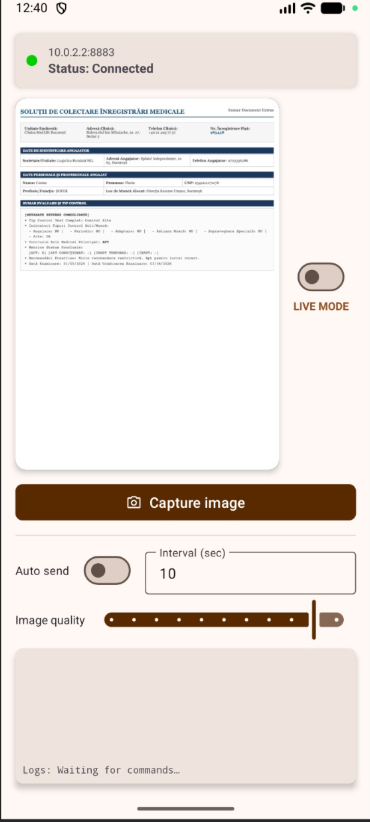
\includegraphics[width=\linewidth]{assets/android_connected.png}
            \\[0.3em]
            \small (a) Connected mode
        \end{minipage}\hfill
        \begin{minipage}[t]{0.4\textwidth}
            \centering
            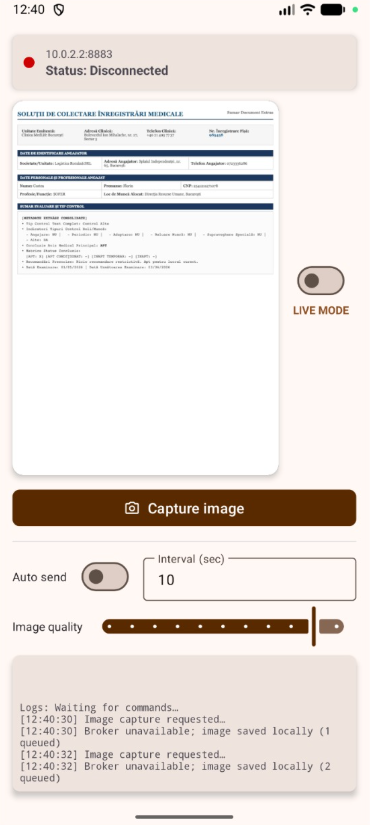
\includegraphics[width=\linewidth]{assets/android_disconnected.png}
            \\[0.3em]
            \small (b) Offline mode
        \end{minipage}
        \caption{Android mobile capture states}
        \label{fig:android-mobile-states}
    \end{figure}

\subsection{Dark Mode}
Dark mode support improves usability in low-light conditions and long-running
monitoring sessions. The interface theme can be switched without affecting
workflow semantics, and key status colors (alerts, warnings, success indicators,
and confidence cues) remain distinguishable in both light and dark modes.


\begin{figure}[H]
    \centering
    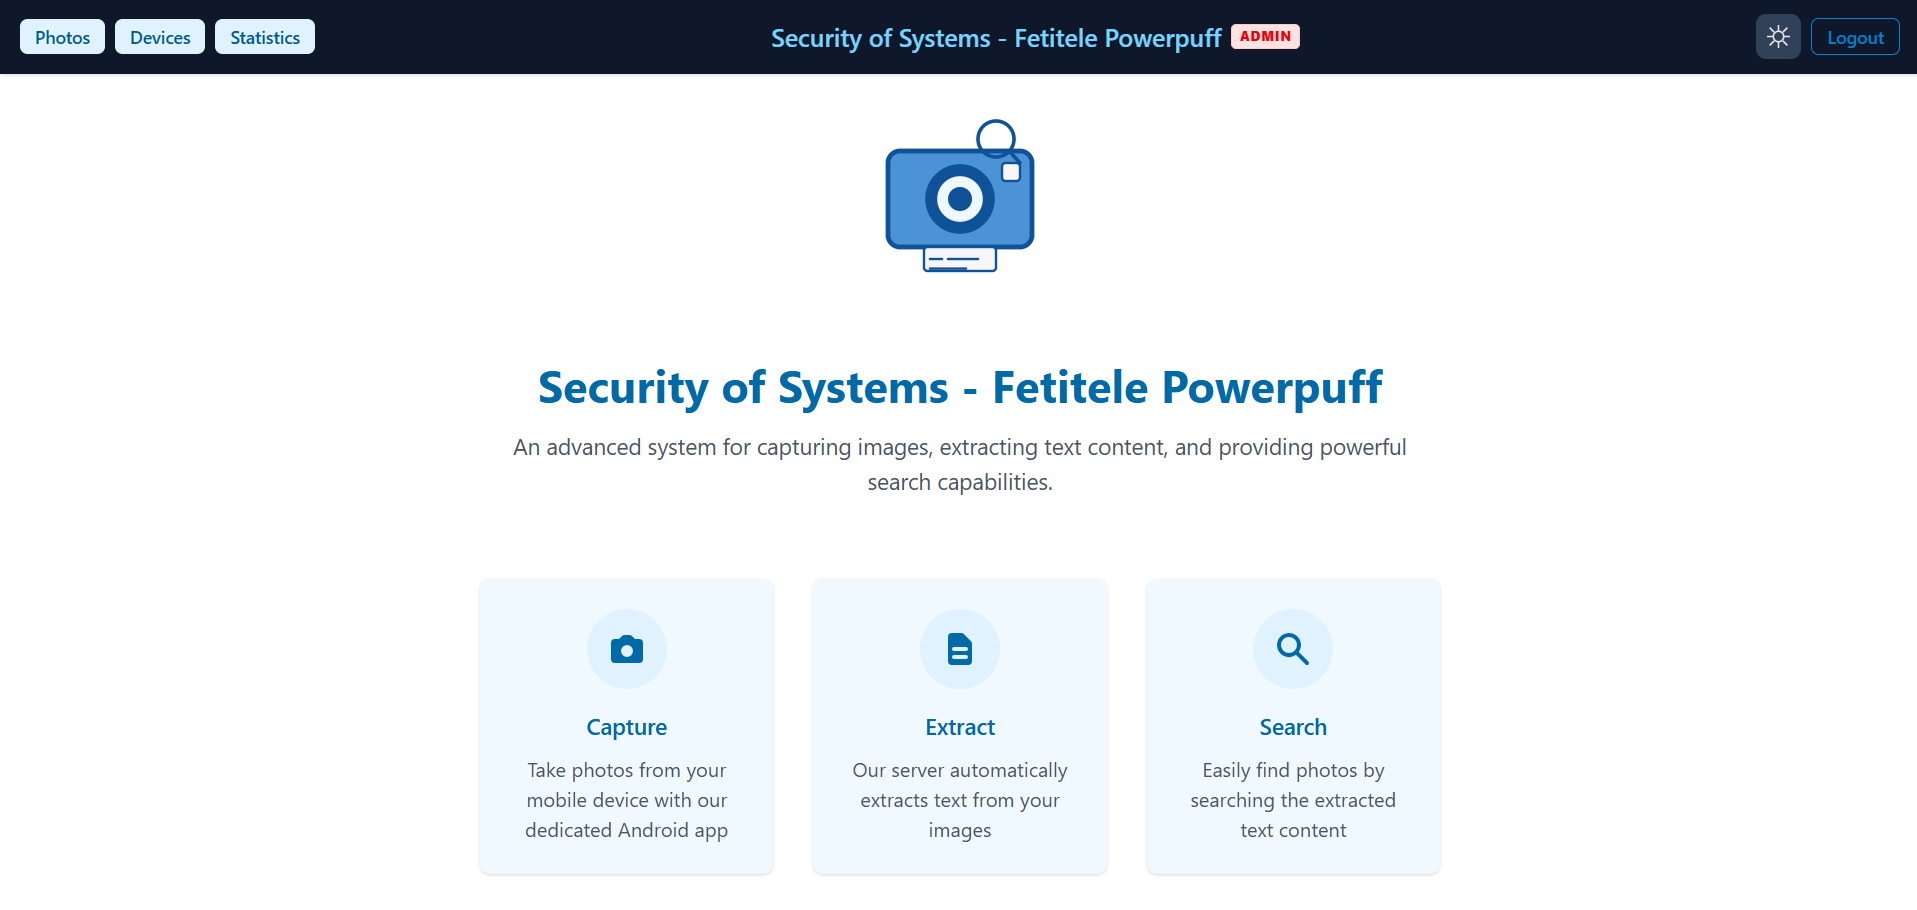
\includegraphics[width=0.9\textwidth]{assets/light.png}
    \caption{Example of light mode page}
    \label{fig:light-mode}
\end{figure}


\begin{figure}[H]
    \centering
    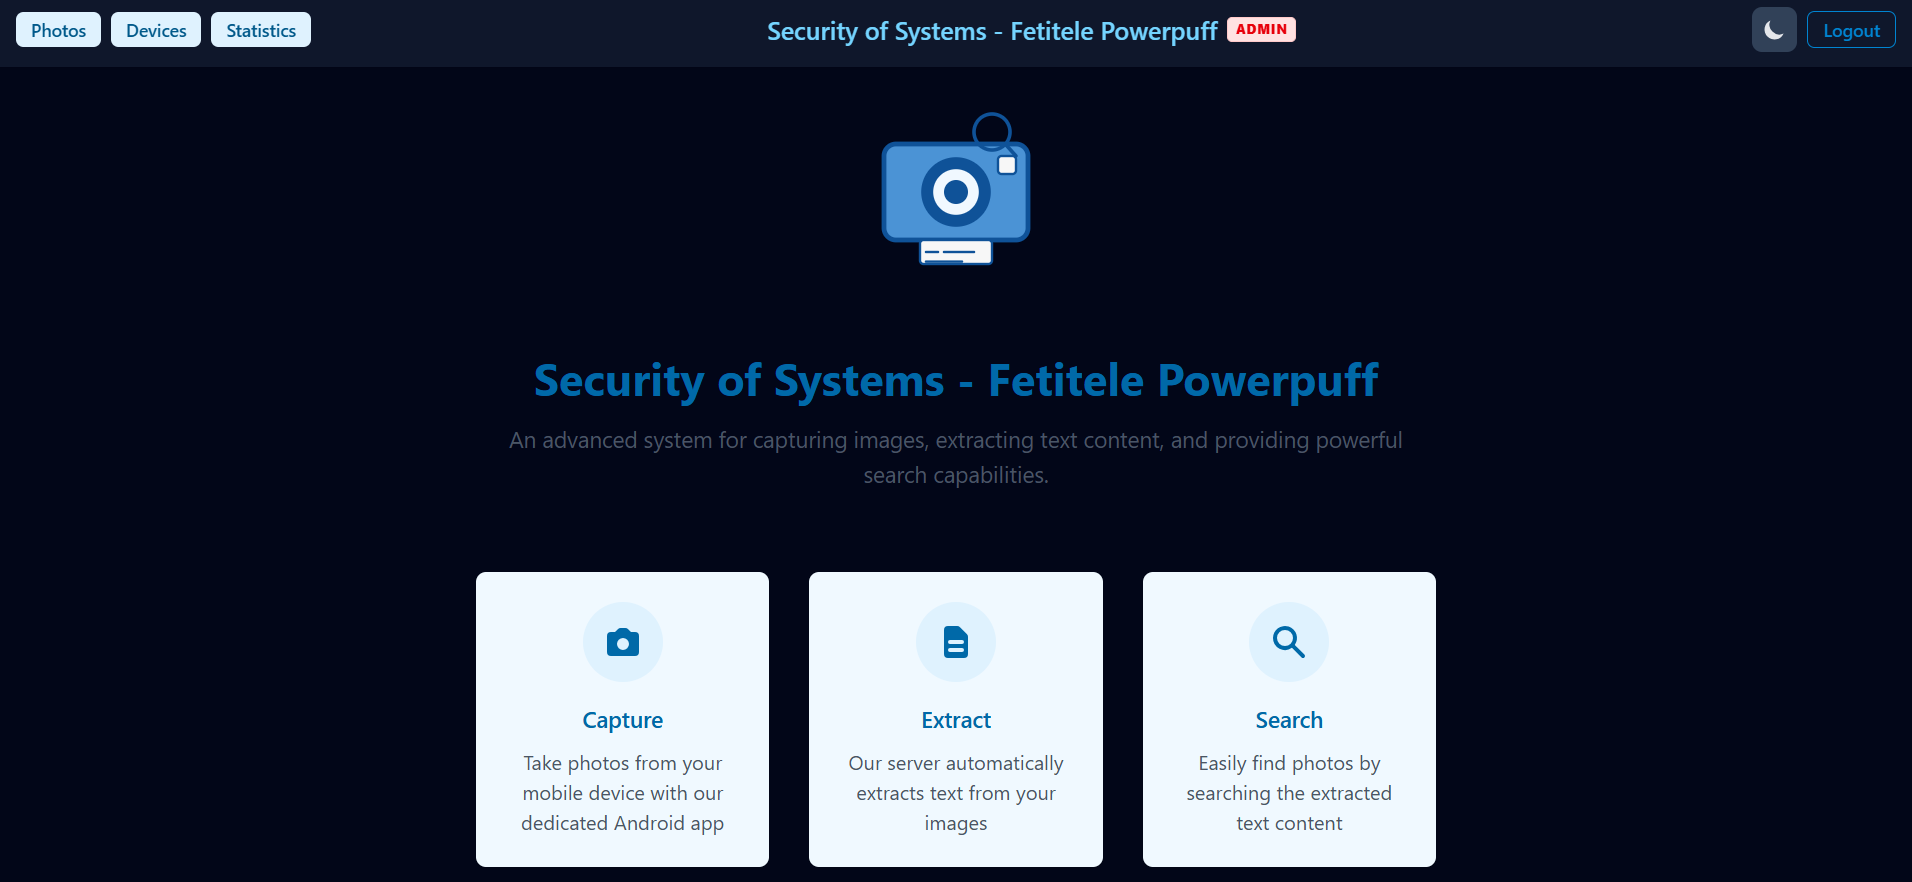
\includegraphics[width=0.9\textwidth]{assets/dark.png}
    \caption{Example of dark mode page}
    \label{fig:dark-mode}
\end{figure}




\section{Documentation}

\subsection{Developer Documentation}
    \subsubsection{System Overview}
    The web platform is composed of five main components:
    \begin{itemize}[leftmargin=*]
        \item React + Vite frontend in \texttt{web/client}.
        \item Go backend API in \texttt{web/server}.
        \item Go gRPC OCR microservice in \texttt{web/ocr-service}.
        \item Mosquitto MQTT broker in \texttt{web/broker}.
        \item PostgreSQL persistence layer.
    \end{itemize}
    The operational data flow starts from mobile capture or web upload,
    continues through the backend and OCR processing pipeline, then passes
    through structured medical parsing and encrypted storage, and finally
    reaches API responses and frontend visualization.

    \subsubsection{Security Architecture}
    Transport security is enforced end-to-end: MQTT communication runs over TLS
    on port 8883 with client certificate validation, backend-to-OCR calls use
    gRPC with mTLS, and web API access is protected through JWT bearer tokens and TLS.
    The broker is hardened against abuse using concrete limits from Mosquitto
    configuration:
    \begin{itemize}[leftmargin=*]
        \item Payload size cap: 10 MB.
        \item Maximum concurrent connections: 100.
        \item Maximum inflight messages per client: 20.
        \item Maximum queued messages per client: 100.
    \end{itemize}

    JWT middleware reads the \texttt{Authorization: Bearer} header, verifies
    signature and expiration, then injects identity attributes (email and role)
    into request context for downstream authorization.

    Role boundaries are explicit:
    \begin{itemize}[leftmargin=*]
        \item Admin-only examples:
        \begin{itemize}[leftmargin=*]
            \item \texttt{GET /users}
            \item \texttt{DELETE /photos/all}
            \item \texttt{GET /photos/anonymized/export}
        \end{itemize}
        \item Non-admin users are scoped to their own records.
    \end{itemize}

    \subsubsection{Backend Structure}
    The backend is organized into focused modules:
    \begin{itemize}[leftmargin=*]
        \item \texttt{routes}: HTTP route handlers.
        \item \texttt{broker}: MQTT message handlers.
        \item \texttt{repository}: data access through GORM.
        \item \texttt{domain}: core models (User, Device, Photo, MedicalData).
        \item \texttt{utils}: authentication, storage, medical parsing helpers.
        \item \texttt{ocr}: gRPC client wrapper.
    \end{itemize}

    Main API groups:
    \begin{itemize}[leftmargin=*]
        \item Authentication:
        \begin{itemize}[leftmargin=*]
            \item \texttt{POST /register}
            \item \texttt{POST /login}
            \item \texttt{GET /profile}
            \item \texttt{GET /users} (admin)
        \end{itemize}
        \item Devices:
        \begin{itemize}[leftmargin=*]
            \item \texttt{GET /devices}
            \item \texttt{POST /devices/claim}
            \item \texttt{POST /devices/switch}
            \item \texttt{POST /devices/command}
        \end{itemize}
        \item Photos and analytics:
        \begin{itemize}[leftmargin=*]
            \item \texttt{GET /photos}
            \item \texttt{POST /photos}
            \item \texttt{PATCH /photos/\{id\}}
            \item \texttt{DELETE /photos/\{id\}}
            \item \texttt{DELETE /photos/all} (admin)
            \item \texttt{GET /photos/performance}
            \item \texttt{GET /photos/medical-insights}
            \item \texttt{GET /photos/anonymized/export} (admin)
        \end{itemize}
        \item System helper:
        \begin{itemize}[leftmargin=*]
            \item \texttt{GET /broker-info}
        \end{itemize}
    \end{itemize}

    \subsubsection{Database and Storage}
    The data model is auto-migrated around three principal entities:
    \begin{itemize}[leftmargin=*]
        \item User
        \item Device
        \item Photo
    \end{itemize}
    Photo persistence follows a split-storage strategy where image binaries are
    stored on disk under
    \texttt{uploads/photos/\{photo\_id\}.jpg}, while metadata and structured
    state are kept in PostgreSQL.

    Sensitive data is protected at rest using AES-GCM encryption:
    \begin{itemize}[leftmargin=*]
        \item OCR free-text content is persisted as \texttt{text\_enc}.
        \item Structured medical content is persisted as
        \texttt{medical\_data\_enc}.
        \item Decryption is performed in the repository layer at read time
        before API response serialization.
    \end{itemize}

    \subsubsection{OCR and Structured Extraction}
    The OCR service is implemented as a Go gRPC server listening on port 50051
    and using Gosseract/Tesseract with English and Romanian language packs.
    OCR responses include:
    \begin{itemize}[leftmargin=*]
        \item \texttt{text}
        \item \texttt{processing\_time\_ms}
        \item \texttt{error} (when relevant)
    \end{itemize}

    After text extraction, the backend checks whether the content resembles a
    medicina muncii certificate and then maps recognized values into a
    structured \texttt{MedicalData} payload. Each extracted field carries:
    \begin{itemize}[leftmargin=*]
        \item a typed value,
        \item confidence (0.0 to 1.0),
        \item optional review flags \texttt{is\_edited} and
        \texttt{is\_validated}.
    \end{itemize}

    Confidence-based review logic in the web UI marks fields for manual review
    when confidence is below 0.95 and the field is neither edited nor
    validated. Users can:
    \begin{itemize}[leftmargin=*]
        \item validate individual fields,
        \item validate all fields,
        \item edit values (edited fields are treated as validated).
    \end{itemize}
    Review changes are persisted through \texttt{PATCH /photos/\{id\}}.

    \subsubsection{Statistics and Reporting}
    The statistics module combines record-level and aggregate reporting for both
    operational monitoring and medical compliance review. Core analytics include
    OCR performance metrics, medical insight summaries, and role-aware report
    endpoints surfaced in the dashboard. Date-range filtering is supported in
    reporting calls, enabling bounded views over selected periods.

    Implemented report capabilities include:
    \begin{itemize}[leftmargin=*]
        \item fit-by-profession analysis,
        \item overdue medical check detection,
        \item monthly compliance trend with completed, fit, overdue, and
        expiring-next-month series,
        \item anonymized dataset export,
        \item fitness diagnosis by profession
    \end{itemize}
    The frontend
    presents these datasets in chart and table form, while anonymized dataset
    export supports privacy-preserving sharing for evaluation and external
    analysis. Admin-only access is preserved for destructive or sensitive
    operations, and non-admin users see data scoped to their own records.

\subsection{User Documentation}

\subsubsection{What the Application Does}
The application helps users capture and upload medical documents, extract key
information automatically, review unclear values, monitor activity through
statistics, and manage connected capture devices. Users with administrator
rights can also access organization-wide views and export anonymized reports.

\subsubsection{Getting Access}
Create an account from the Register page, then sign in from the Login page
using your email and password. After login, protected pages become available.
Regular users see their own data, while administrators can access global data
and additional management actions.

\subsubsection{Mobile App Guide}
At first launch, users configure connection settings and sign in. The mobile
dashboard supports manual capture, continuous live capture, periodic automatic
send, and image-quality adjustments. If connectivity drops, the app keeps new
captures safely in a local queue and sends them automatically when the
connection is restored.

\subsubsection{Devices Page}
The Devices page is used to monitor connected devices and trigger capture
actions remotely. Users can start a capture, start live mode, or stop live
mode, and can also verify current connection state.

\subsubsection{Photos Page}
The Photos page allows searching and filtering records, uploading new images,
and opening entries for review. Users can inspect extracted fields, validate
values, and correct information when needed. Individual photos can be removed,
while full bulk deletion remains an admin-only operation.

\subsubsection{Statistics Page}
The Statistics page presents activity summaries, medical-status distributions,
performance indicators, and renewal-related insights. Date filters can be used
to focus results on a selected period. If upcoming expirations are detected, an
alert is displayed and can be snoozed temporarily.

\subsubsection{Anonymized Report Export}
Administrators can download anonymized reports for analysis and presentation.
These exports are intended for sharing trends and outcomes without exposing
direct personal identifiers.



\section{Execution}
\subsection{CI/CD}
\subsubsection{Web CI Workflow}
The web pipeline is implemented in
\path{.github/workflows/ci-web.yml} (workflow name: CI). It is triggered on
push to \texttt{main}, pull requests targeting \texttt{main}, and through
\texttt{workflow\_call} so it can be reused by other workflows.

Main validation steps include:
\begin{itemize}[leftmargin=*]
    \item Go backend build and tests in \texttt{web/server}.
    \item Frontend lint/build in \texttt{web/client}.
    \item Docker build for the API image.
    \item Artifact upload for \texttt{go-test-results} and
    \texttt{go-coverage}.
\end{itemize}

\subsubsection{Mobile CI/CD Workflow}
The mobile pipeline is implemented in
\texttt{.github/workflows/ci-mobile.yml} (workflow name: Mobile CI/CD). It is
triggered on push to \texttt{main}, push on version tags
(\texttt{v*}), pull requests targeting \texttt{main}, and
\texttt{workflow\_call}. Path filters include the mobile module and mTLS
generation scripts.

The \texttt{mobile\_checks} job performs JDK 17 setup, Android mTLS resource
generation, lint, Semgrep static analysis, unit tests, instrumented tests on
an emulator (API 31), and debug APK build, then uploads
\texttt{mobile-test-reports} and \texttt{app-debug-apk} artifacts. The
\texttt{release} job runs only for tag refs, downloads the APK artifact, and
publishes it in a GitHub Release.

\subsubsection{CodeQL Advanced Workflow}
CodeQL analysis is implemented in
\texttt{.github/workflows/codeql.yml} (workflow name: CodeQL Advanced),
triggered on push to \texttt{main} and pull requests targeting
\texttt{main}. The language matrix includes Go on autobuild and Java/Kotlin on manual build path.

The workflow initializes CodeQL with security-extended and
security-and-quality query suites, prepares Android prerequisites where
needed, runs analysis, and publishes code scanning results.

\subsubsection{SBOM Update Automation}
SBOM maintenance is automated in
\path{.github/workflows/update-sbom-readme.yml} (workflow name: Update SBOM
README). It runs on \texttt{main} pushes that match dependency/SBOM path
filters and can also be launched manually via \texttt{workflow\_dispatch}.

The workflow executes \path{web/scripts/update-sbom-readme.sh}, regenerates
\path{web/server/sbom.cdx.json} and
\path{web/ocr-service/sbom.cdx.json}, updates the SBOM snapshot in the root
README, and commits/pushes changes automatically when differences are detected.

\subsubsection{AI Governance and Quarantine Promotion}
AI governance and quarantine promotion are intentionally coupled in the
delivery process. Governance rules (architectural guardrails, RBAC-like zone
restrictions, forbidden-path boundaries, and audit logging) constrain what
AI-assisted changes can modify and require traceability for every automation
step.

Promotion is implemented in
\texttt{.github/workflows/promote-quarantine.yml} (workflow name: AI
Quarantine Promotion), triggered on pushes to
\texttt{quarantine/**}. The workflow calls reusable web and mobile validation
workflows (\texttt{ci-web.yml} and \texttt{ci-mobile.yml}). Only when these
validations pass does the automation create/promote the PR to
\texttt{main}. Audit evidence from \texttt{ai-governance/audit.log} is attached
to the PR body, preserving a human-reviewable governance trail.

The flow of operations is aligned according to the following steps:
\begin{enumerate}[leftmargin=*]
    \item Plan: AI orchestrator receives task and logs rationale.
    \item Govern: Capability gateway enforces write zones and forbidden paths.
    \item Execute: Changes are staged on quarantine/* branches and validated by
    CI workflows.
    \item Verify: Web and mobile pipelines must pass before automated PR
    promotion.
    \item Record: Audit log is attached in promotion PR body for traceability
    evidence.
\end{enumerate}

This ensures the practice of human-in-the-loop, risk to main branch is reduced 
by quarantine measures, while artifacts and workflow logs provide traceability required for auditing.


\section{Security and Compliance}

\subsection{Threat Modeling and Mitigations}
Threats such as untrusted image payloads, OCR RCE risk, PHI leakage in transit and at rest,
unauthorized access to medical records, CI/CD bypass by autonomous agents and 
DoS risk on MQTT ingestion were addressed through numerous security measures.
Mitigations include the following, as well as many others:
\begin{itemize}[leftmargin=*]
    \item OCR service runs in a constrained container setup with read-only root,
    tmpfs, no-new-privileges, non-root runtime, and distroless final
    image.
    \item mTLS is used for MQTT and OCR gRPC service-to-service communication.
    \item HTTPS endpoint is exposed for login/API access.
    \item Medical text and structured medical data are encrypted before DB
    persistence (AES-GCM service in repository layer).
    \item JWT-based authentication and role checks are used on protected routes.
    \item MQTT broker limits include:
    \begin{itemize}[leftmargin=*]
        \item \texttt{message\_size\_limit}
        \item \texttt{max\_connections}
        \item \texttt{max\_inflight\_messages}
        \item \texttt{max\_queued\_messages}
    \end{itemize}
    \item AI governance enforces RBAC-style write zones and quarantine branch
    strategy.
\end{itemize}


\begin{figure}[H]
    \centering
    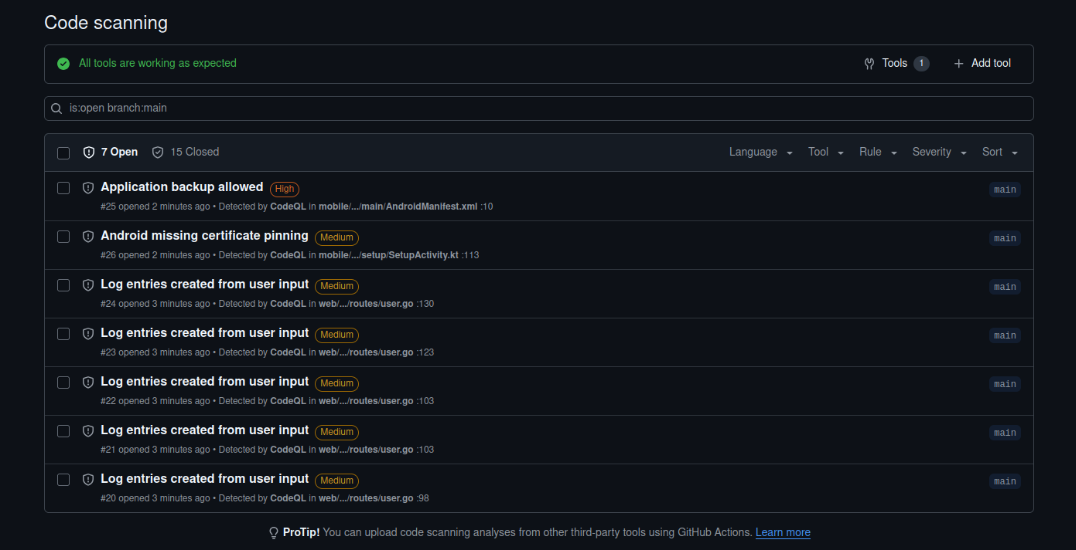
\includegraphics[width=0.9\textwidth]{assets/codeql.png}
    \caption{CodeQL Output}
    \label{fig:codeql-output}
\end{figure}

In order to automate threat modeling, CodeQL tool was used for static code analysis. 
At every new PR, the tool 
runs for each line added. CodeQL generates and reports issues. In figure 
\ref{fig:codeql-output}, it can be seen that the Pull Requests have certain issues. The Static 
Analysis Summary is provided by the CodeQL tool and it uses the 
security-extended and security-and-quality query packs. We use this 
tool because it is more suitable for the go language. Not only that, 
but it found an Easter egg that could turn critical for Kotlin too.

\begin{figure}[H]
    \centering
    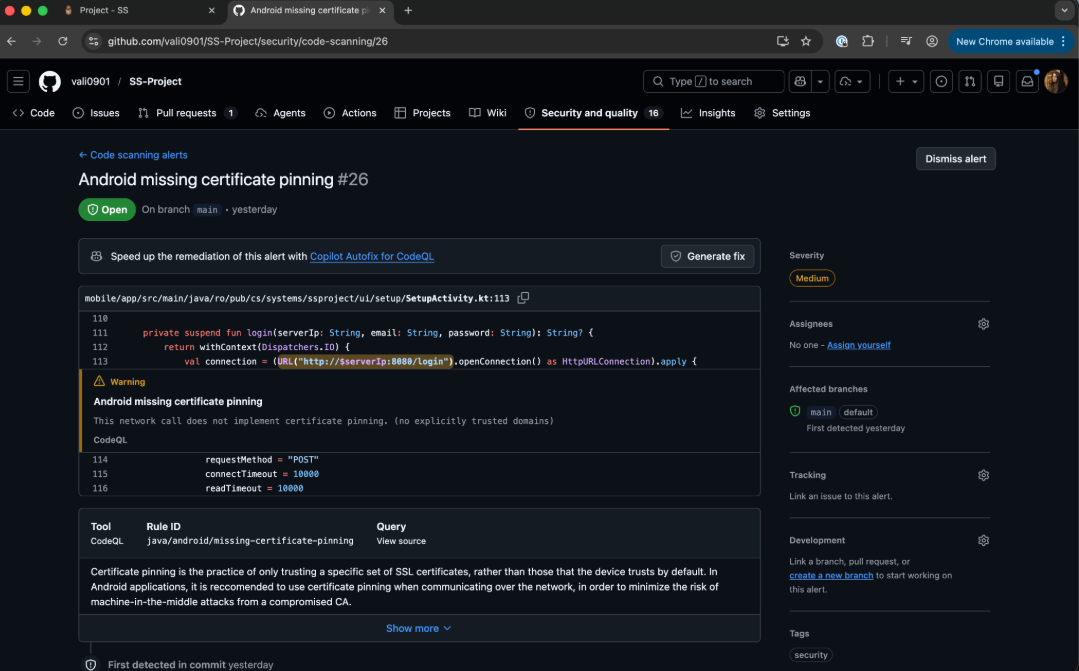
\includegraphics[width=0.9\textwidth]{assets/android_bug.png}
    \caption{Kotlin issue reported by CodeQL}
    \label{fig:android-codeql-issue}
\end{figure}

\subsection{MISRA / CERT Compliance}
Project languages are primarily Go, TypeScript, Kotlin, and Python. MISRA C is
not directly applicable to the main codebase. Instead, we adapted by using more 
suitable solutions, such as CodeQL for advanced security analysis for Go and Java/Kotlin,
Semgrep static checks for mobile pipeline.
Standards such as non-root containers, key/cert secret mounts, and explicit TLS
validation, password hashing with bcrypt and token validation middleware,
were also upheld.

\subsection{Testing and Coverage}
\subsubsection{Testing}
Testing is accomplished on all fronts, the project accompassing Go 
backend unit tests for routes, auth, broker handlers, performance/report 
logic, as well as Android unit tests and instrumented tests in CI and 
frontend lint/build checks in CI.

\subsubsection{Coverage}

\begin{figure}[H]
    \centering
    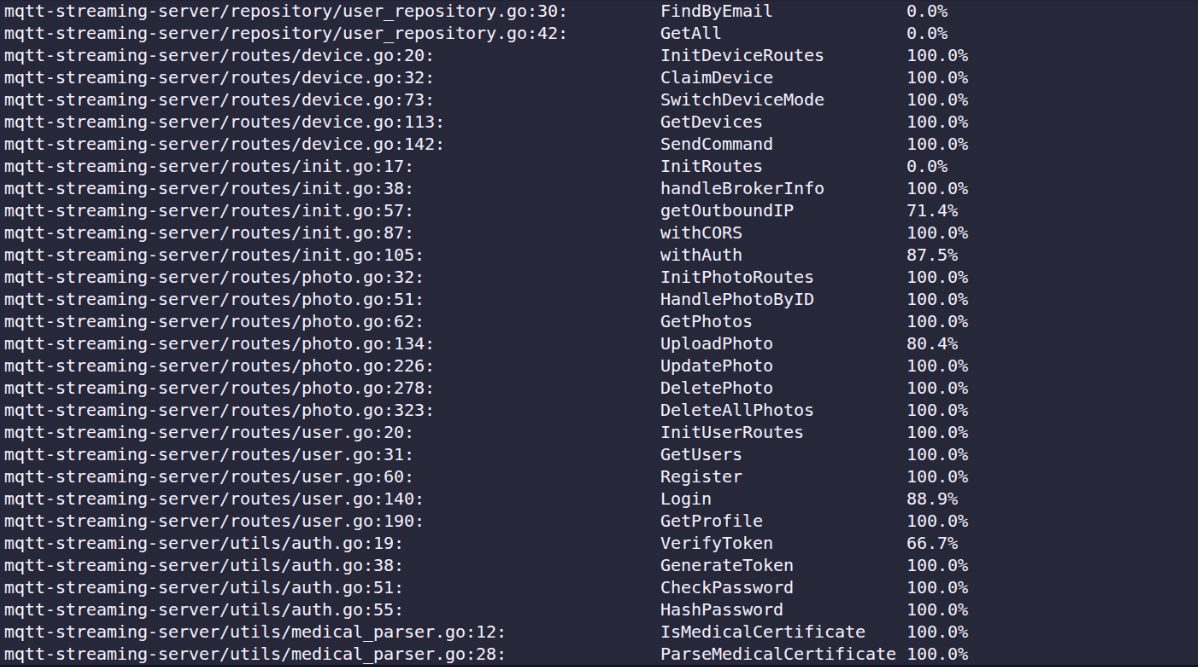
\includegraphics[width=0.9\textwidth]{assets/test_coverage1.png}
    \caption{Test coverage (1)}
    \label{fig:test-coverage-1}
\end{figure}

\begin{figure}[H]
    \centering
    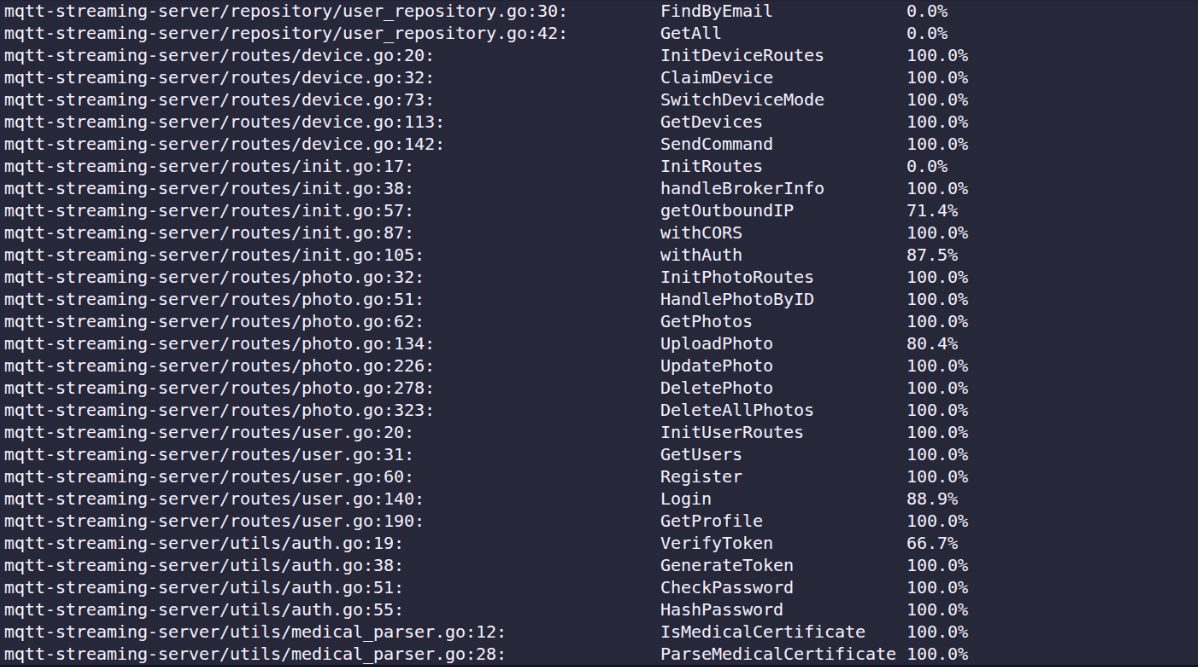
\includegraphics[width=0.9\textwidth]{assets/test_coverage1.png}
    \caption{Test coverage (2)}
    \label{fig:test-coverage-2}
\end{figure}

The go cover tool is used for finding the test coverage of the project. We tried to 
focus on the most important sections to reach a high score in order to obtain a 
more secure project. As it can be seen in the pictures above, almost every 
important functionality (device, user and photo) has 100\% code coverage testing. 
We integrated the code coverage test in the CI of the web app. The fuzzing 
testing is integrated in the codes written for testing that introduce malformed 
input in order to see that our web app is returning the good error http code (400 bad request).

The coverage results shown in Figures \ref{fig:test-coverage-1} and
\ref{fig:test-coverage-2} indicate that the most critical modules have strong
automated test coverage.

\subsection{SBOM and Dependencies}
CycloneDX SBOM is generated for web and OCR services with an automated update
workflow which commits refreshed artifacts. The maintained SBOM summary 
can be used to track dependency inventory for auditing purposes.

\subsection{Fixing Own Vulnerabilities}
Among the fixed security issues, the following can be counted:
\begin{enumerate}[leftmargin=*]
    \item Dependabot upgraded vulnerable frontend packages in \textit{yarn.lock}, 
    \textit{react-router}, \textit{react-router-dom}, \textit{minimatch}, \textit{picomatch}, 
    and \textit{set-cookie-parser}.
    \item CodeQL-related remediations:
    \begin{itemize}[leftmargin=*]
        \item Disabled Android app backup and excluded app data from
        backup/transfer.
        \item Replaced Android HTTP login with HTTPS.
        \item Added Android network security config for trusted CA and
        generated certificate pinning.
        \item Removed raw user-controlled email values from backend auth logs.
    \end{itemize}
\end{enumerate}

Besides those, the following can be counted towards hardening the application:
\begin{enumerate}[leftmargin=*]
    \item HTTPS listener for the Go API and enabled Renovate.
    \item Encryption-at-rest for OCR text and medical structured fields.
    \item OCR isolation with distroless runtime and restrictive container
    controls.
    \item JWT auth + role-gated endpoints for admin-only reports and exports.
    \item MQTT broker resource limits to reduce DoS impact.
    \item Quarantine-gated AI changes with mandatory CI validation before PR
    promotion.
\end{enumerate}

\subsection{Reporting Peer Issues}

Evidence for a reported peer-project issue is included below.

\begin{figure}[H]
    \centering
    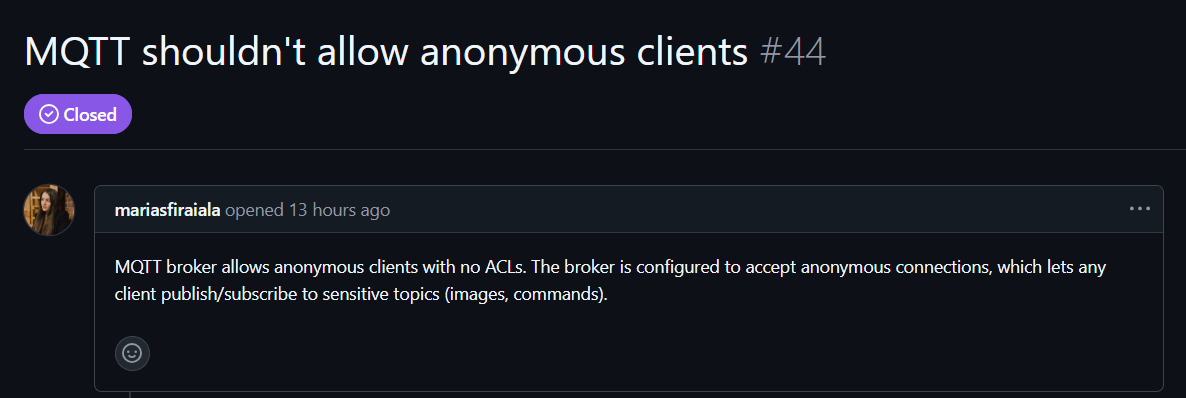
\includegraphics[width=0.9\textwidth]{assets/peer_issue_report.png}
    \caption{Peer issue report evidence}
    \label{fig:peer-issue-report}
\end{figure}

\newpage

\section{Medical Reports}


\subsection*{Report 1: Total Processed Medical Documents}
\begin{figure}[H]
    \centering
    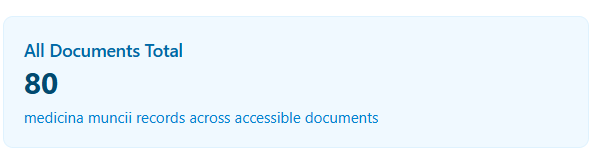
\includegraphics[width=0.5\textwidth]{assets/documents_total.png}
    \caption{Total of documents submitted}
    \label{fig:report-total-documents}
\end{figure}

\subsection*{Report 2: Medical Opinion Distribution}
\begin{figure}[H]
    \centering
    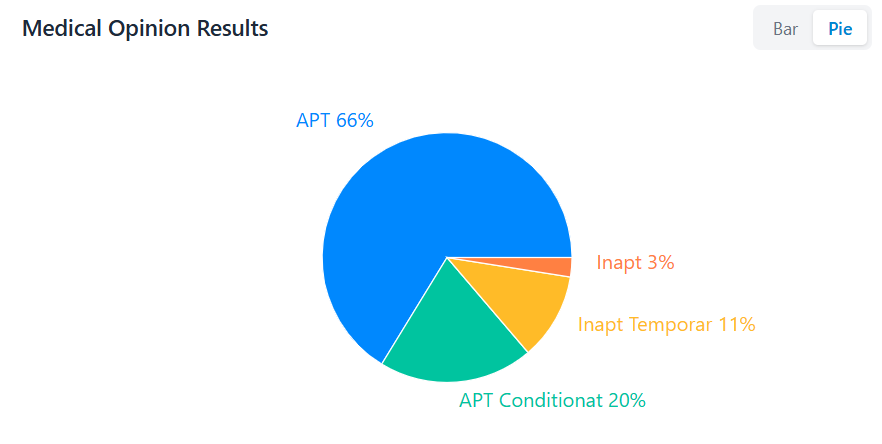
\includegraphics[width=0.5\textwidth]{assets/medical_opinion.png}
    \caption{Distribution of medical opinions across documents}
    \label{fig:report-medical-opinion}
\end{figure}

\subsection*{Report 3: Control Type Distribution}
\begin{figure}[H]
    \centering
    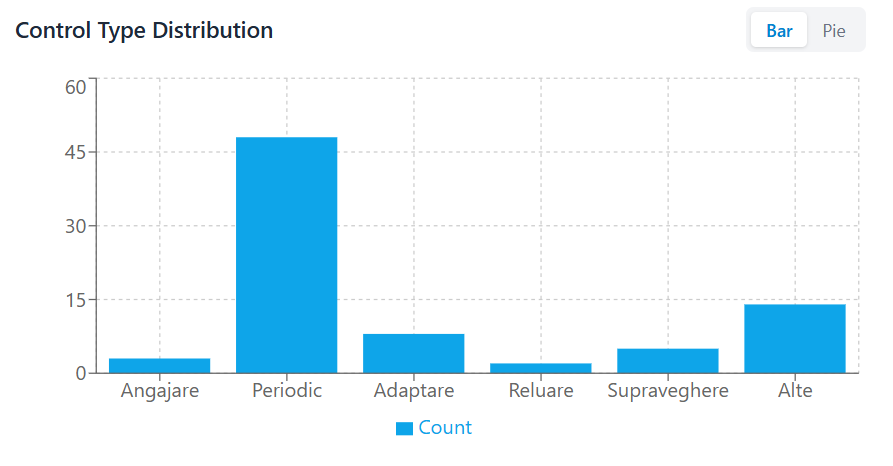
\includegraphics[width=0.5\textwidth]{assets/control_type.png}
    \caption{Distribution of control types across data}
    \label{fig:report-control-type}
\end{figure}

\subsection*{Report 4: Documents Issued in Last 30 Days}
\begin{figure}[H]
    \centering
    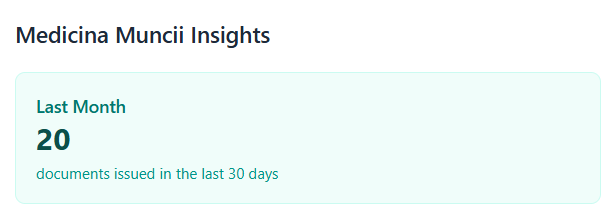
\includegraphics[width=0.5\textwidth]{assets/last_30_days.png}
    \caption{Total of documents submitted within the last 30 days}
    \label{fig:report-last-30-days}
\end{figure}

\subsection*{Report 5: Expiring Next Month}
\begin{figure}[H]
    \centering
    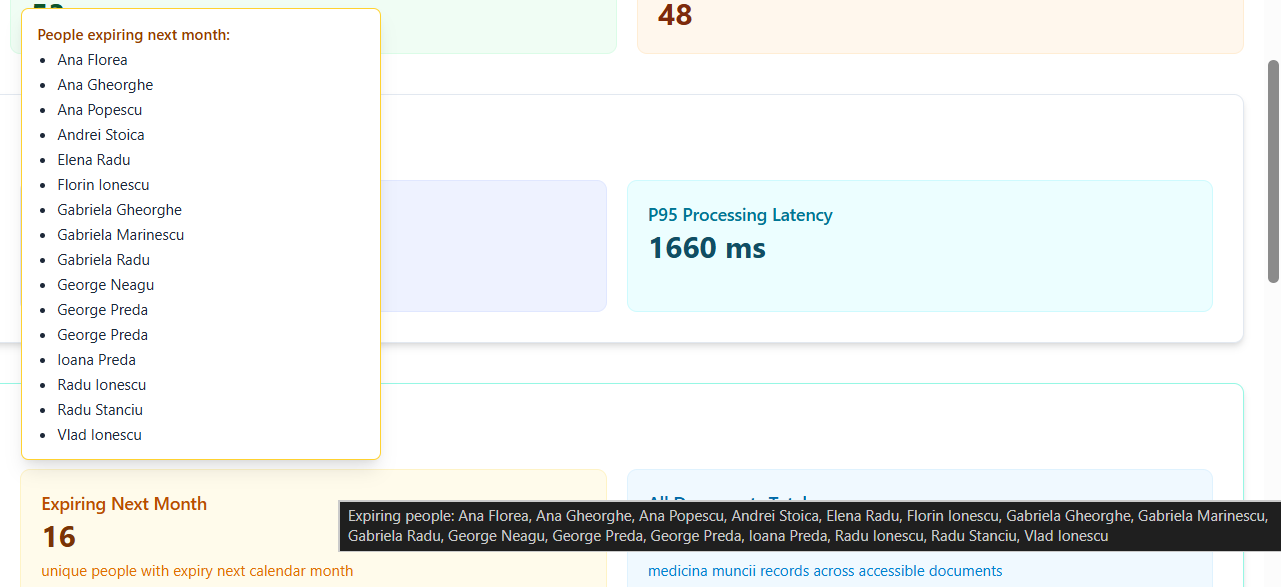
\includegraphics[width=0.9\textwidth]{assets/next_month_expiry.png}
    \caption{People whose control expiration date is within the next month}
    \label{fig:report-next-month-expiry}
\end{figure}

\subsection*{Report 6: Overdue Medical Checks}
\begin{figure}[H]
    \centering
    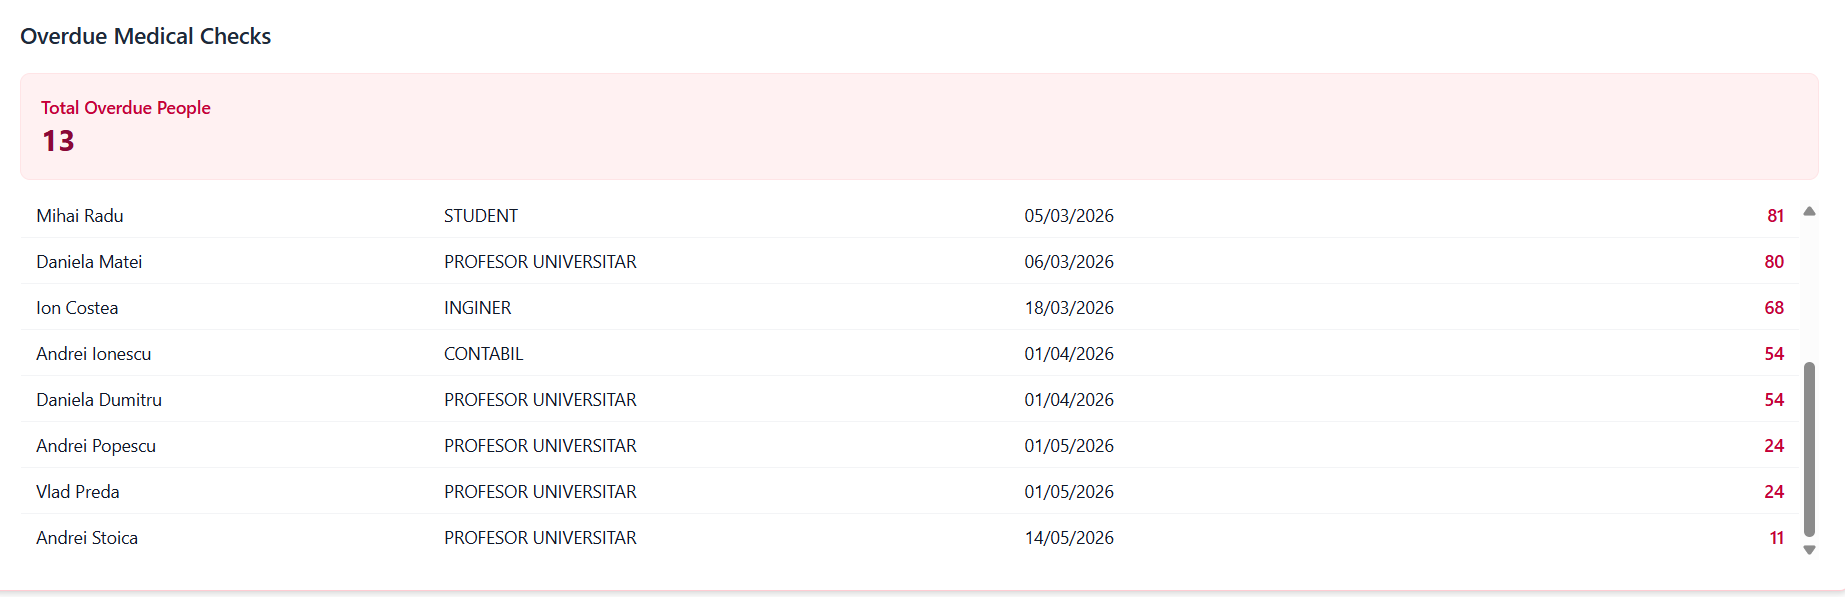
\includegraphics[width=0.9\textwidth]{assets/overdue.png}
    \caption{People with overdue medical checks}
    \label{fig:report-overdue}
\end{figure}
\subsection*{Report 7: Fit Rate by Profession}
\begin{figure}[H]
    \centering
    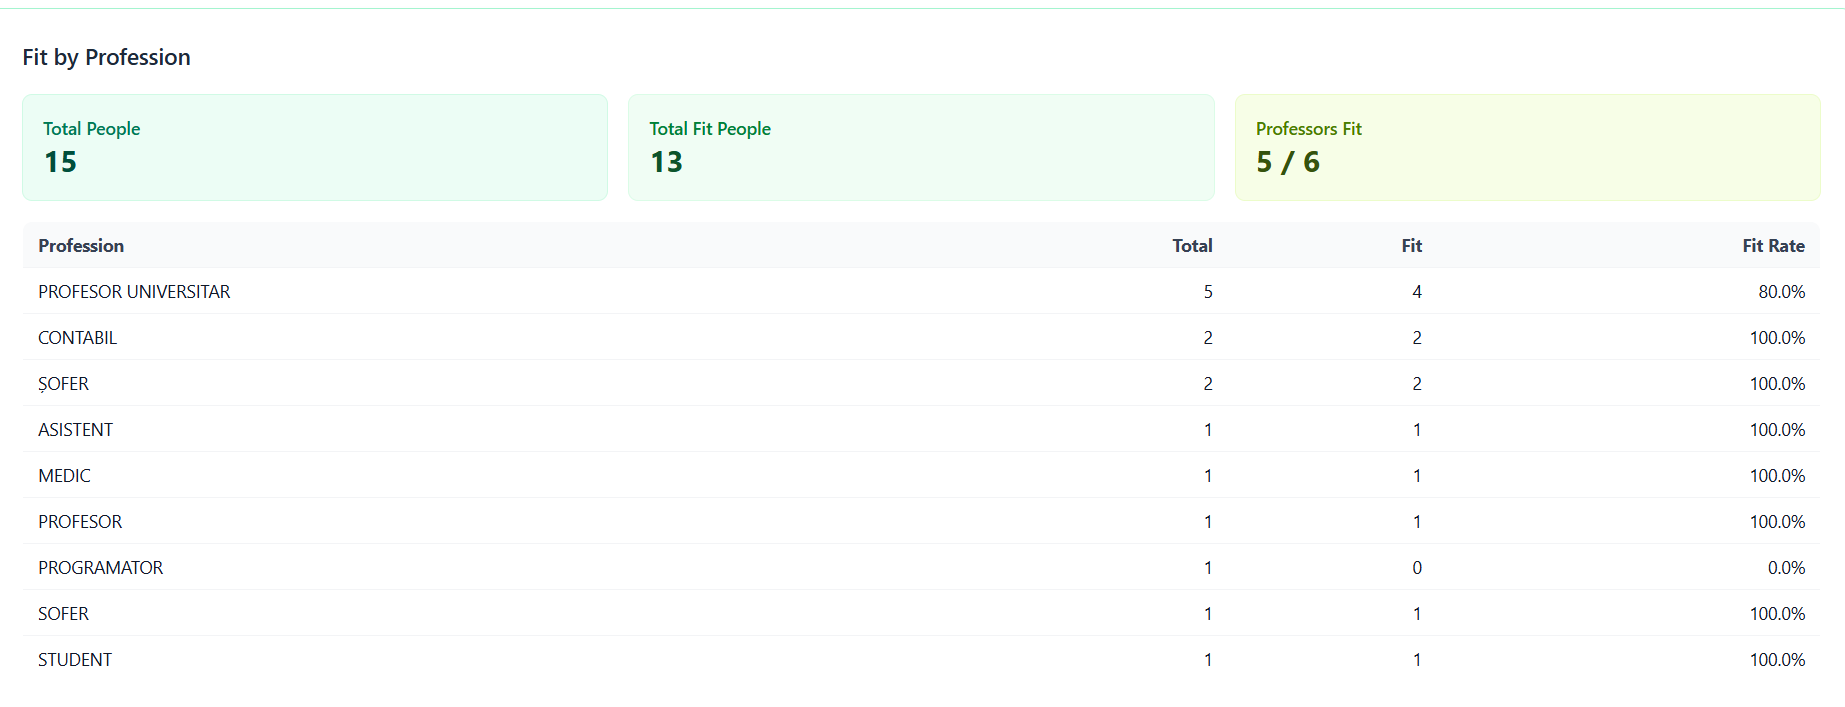
\includegraphics[width=0.9\textwidth]{assets/fit_by_profession.png}
    \caption{Fit rate distributed by profession}
    \label{fig:report-fit-by-profession}
\end{figure}

\subsection*{Report 8: Monthly Compliance Trend}
\begin{figure}[H]
    \centering
    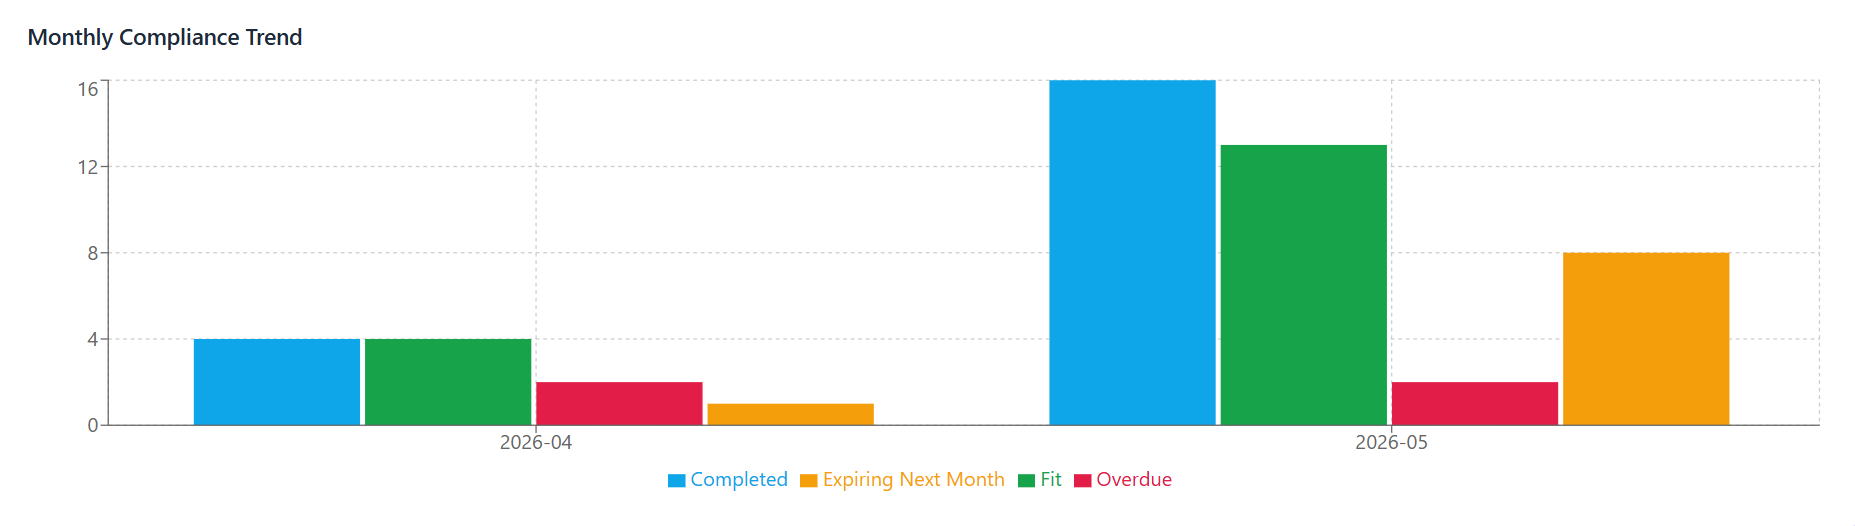
\includegraphics[width=0.9\textwidth]{assets/monthly_trend.png}
    \caption{Trend of fit diagnosis distributed monthly}
    \label{fig:report-monthly-trend}
\end{figure}

\section{Team Contributions}

Contribution table based on repository history is the following, bearing in mind that the
contributions were not not limited to Github code and may vary based on personal habits
such as squashing or not squashing one's commits:

\begin{table}[H]
    \centering
    
\begin{tabular}{l r r r}
    \toprule
   \textbf{Team Member} & \textbf{Lines Added} & \textbf{Lines Removed} &
   \textbf{Number of Commits} \\
    \midrule
    Andrei Airinei & 5961 & 6896 & 68 \\
    Ecaterina-Ioana Minca & 15142 & 593 & 29 \\
    Maria Teodor & 6457 & 1296 & 21 \\
    Maria Sfiraiala & 1415 & 345 & 15 \\
    Valentin-Ionut Bobaru & 3257 & 130 & 13 \\
    \bottomrule
\end{tabular}
\caption{Git statistics per team member}
\end{table}

In order to organize better, tasks were proposed and assigned on a voluntary basis 
using the Trello platform. Some of the tasks and their assignee can be 
observed in Figure \ref{fig:trello-board}.
\begin{figure}[H]
    \centering
    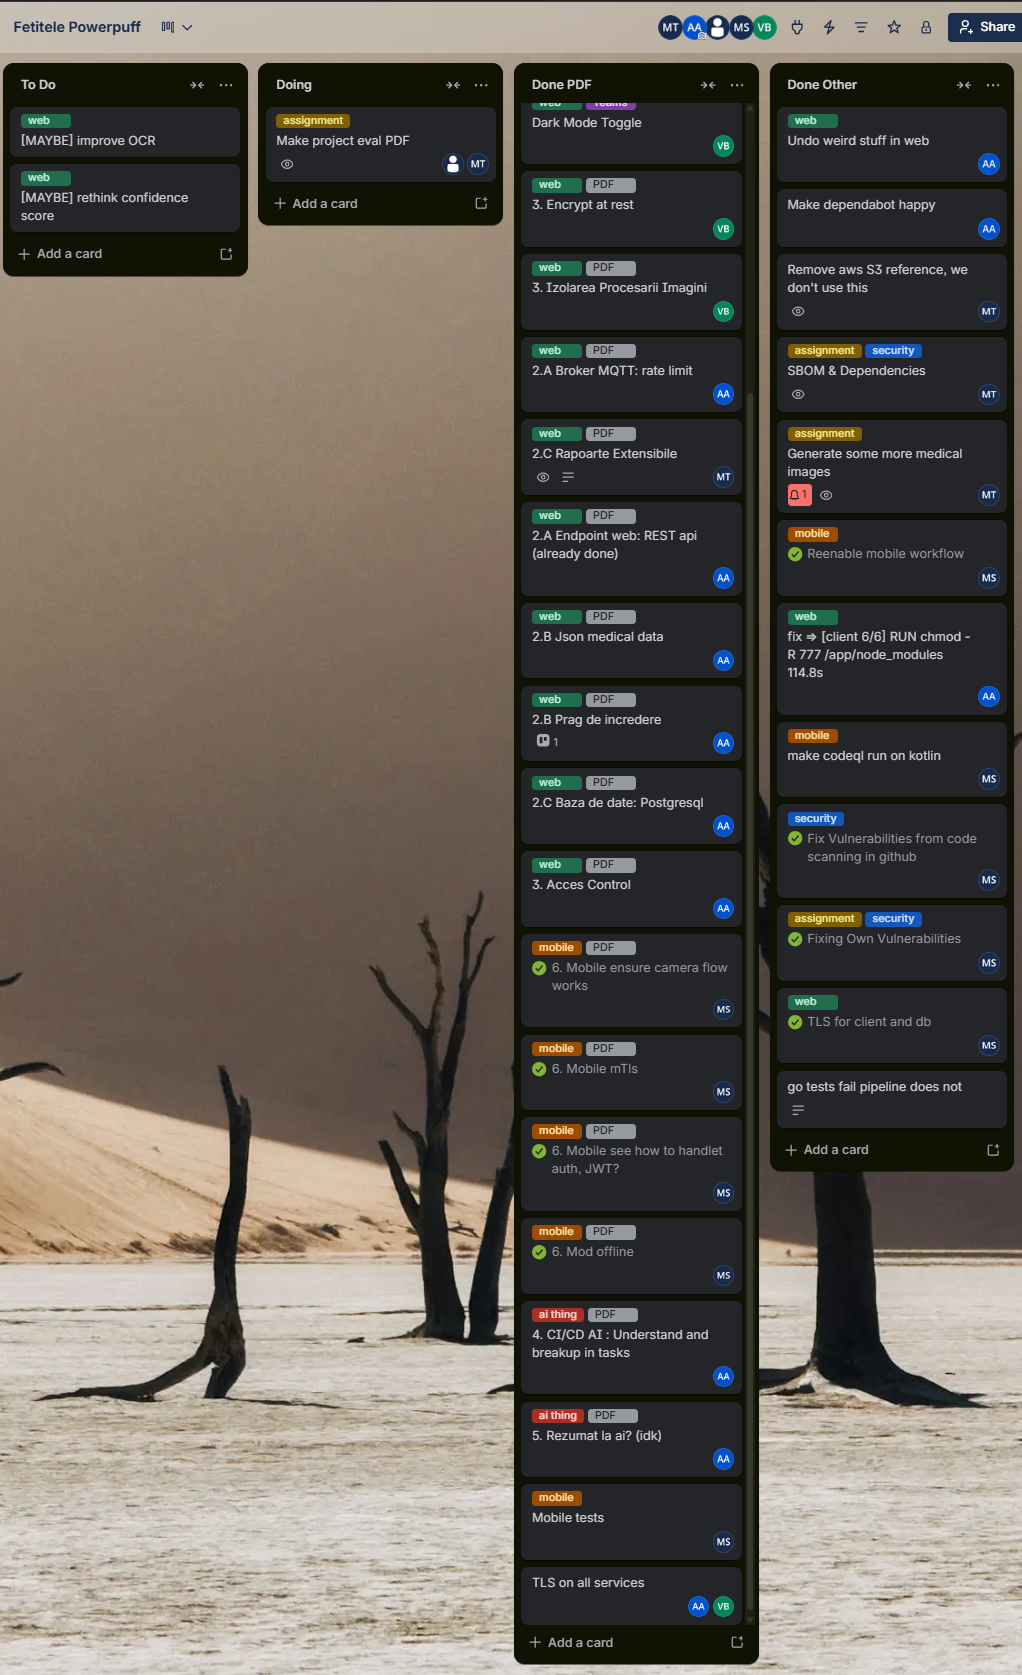
\includegraphics[width=0.7\textwidth]{assets/trello.png}
    \caption{Trello Board for Tasks}
    \label{fig:trello-board}
\end{figure}

\newpage

\section{OSSF Criticality Score}
Figure \ref{fig:ossf-criticality} presents a screenshot of the output of running OSSF Criticality score tool 
using \texttt{original\_pike.yml}.
\begin{figure}[H]
    \centering
    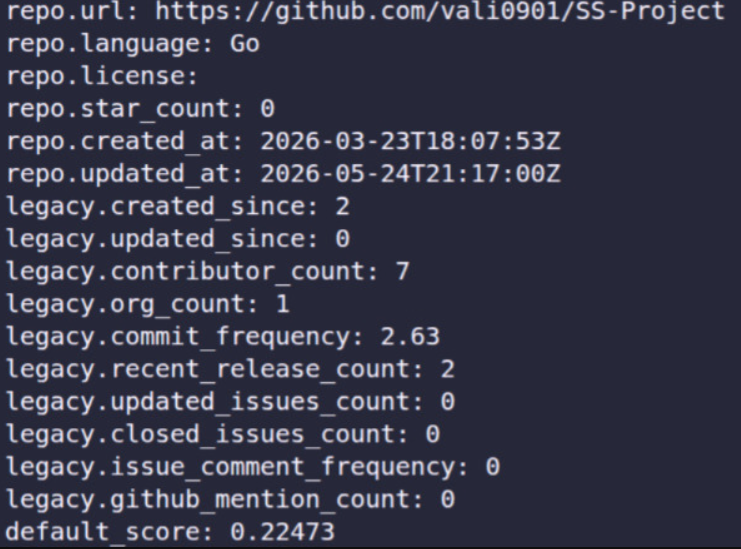
\includegraphics[width=0.9\textwidth]{assets/ossf.png}
    \caption{OSSF Criticality Score}
    \label{fig:ossf-criticality}
\end{figure}

\end{document}
